\documentclass[12pt]{report}

\usepackage[latin1]{inputenc}
\usepackage[Glenn]{fncychap}
\usepackage{graphicx}
\usepackage{tikz}
\usepackage[hidelinks]{hyperref}
\usepackage{float}
\usepackage{mathtools}
\usepackage[toc,page]{appendix}
%\usepackage{cite}
\usepackage{algorithm}
\usepackage{algorithmicx}
\usepackage{algpseudocode}
\usepackage{ifthen}

\newcommand{\argmax}[1]{\underset{#1}{\operatorname{arg}\,\operatorname{max}}\;}
\newcommand{\argmin}[1]{\underset{#1}{\operatorname{arg}
\,\operatorname{min}}\;}

%Figures aliases
%Usage: \image{path}{width}{caption}{label}
%Try to allways use \image and let latex fix positioning of figures.
%By passing 'null' as width the latex will use the figures default size
%Do however but the command at the wanted position within the text, 
%if we at a later stage want to fix the positioning of all images it could be done by rewriting this alias.
\newcommand{\image}[4]{
	\ifthenelse{\equal{false}{true}}{%true - true => latex fixes positioning, mismatch => forced positioning by float
		\begin{figure}[ht]
			\centering
			\insertImage{#1}{#2}
			\caption{#3}
			\label{#4}
		\end{figure}
	}{
		\imageHere{#1}{#2}{#3}{#4}
	}	
}
\newcommand{\imageHere}[4]{
	\begin{figure}[H]
		\centering
		\insertImage{#1}{#2}
		\caption{#3}
		\label{#4}
	\end{figure}
}
%Helper function, do not use
\newcommand{\insertImage}[2]{
	\ifthenelse{\equal{#2}{null}}{
		\includegraphics{#1}
	}{
		\includegraphics[width=#2]{#1}
	}
}


%%Force correct display style for math environments
\everymath{\displaystyle}

\begin{document}

\begin{titlepage}
	\noindent {\large \textbf{\thesisAuthor}}
	\vspace{2cm}

	\noindent {\Huge \thesisTitle}
	\vspace{2cm}
	
	\noindent \thesisType, \thesisDate 
	\vspace{2cm}

	\noindent Artificial Intelligence Group\\ Department of Computer and Information Science\\ Faculty of Information Technology, Mathematics and Electrical Engineering\\

	\vfill
	\begin{center}
		
\includegraphics[width=3cm]{images/NTNUlogo.pdf}
	\end{center}
\end{titlepage}

%\thispagestyle{empty}
%\mbox{}\\[6pc]
%\begin{center}
%	\Large{TDT4501 Datateknikk, Master thesis}\\
%	\large{Spring 2014}\\[4pc]
%	\Huge{Educational Robotics}\\[2pc]
%	
%	\Large{Jan Tore St�lsvik}\\[1pc]
%	\Large{Nicklas Utgaard}\\[4pc]
%	%\Large{\today}\\[2pc]
	
	%PROJECT THESIS\\
%	Department of Computer Science,\\
%	NTNU, Trondheim\\[6pc]
	
%	\today
%\end{center}
%\vfill

%\noindent Supervisor 1: Pauline Haddow

%\noindent Supervisor 2: Guttorm Sindre
\setcounter{page}{0}
\pagenumbering{roman}
\section*{Abstract}
In the later years robotics has seen a huge increase within domestic use, and have now become an affordable tool in the daily life of most people.
The goal of this project was to investigate the differences between a physical and virtual robot in terms of increased content knowledge, learning motivation, and interest in science, technology, engineering and mathematics (STEM).
	%The goal of this thesis is to look into how robotics can be combined with the early education of children in K-12, in order to increase content knowledge, motivate learning and generate more interest within the STEM fields.
To investigate this we conducted an experiment at Trondheim'm International School (THIS), using a quasi-experimental setup with two treatment group, virtual and physical robot. 
	%To investigate the applicability of robotics an experiment was conducted at Trondheim's International School (THIS) 
The results showed that there does not exist a statistically significant difference in content knowledge gain, motivation or interest between the robotics group and the simulator group. 

\newpage
\section*{Sammendrag}
 De siste årene har roboter økt i popularitet innenfor vanlige hushold, og har kommet ned på ett prisnivå som gjør robotene tilgjengelig for folk flest.
Målet med denne oppgaven var å undersøke forskjellene mellom en fysisk og virtuell robot med tanke på å øke kunnskapsnivået, motivasjonen og interessen for vitenskap, teknologi, ingeniørskap og matematikk (STEM).
For å undersøke dette utførte we ett eksperiment hos Trondheim's International School (THIS), hvor vi brukte ett kvasieksperimentelt oppsett med to behandlingsgrupper, virtuell og fysisk robot.
Resultatene viste at det ikke fantes noen statistisk signifikant forskjell i økning av kunnskapsnivå, motivasjon eller interesse mellom robot gruppen og simulator gruppen.
\section*{Preface}
	This pre-master's project was carried out within the Information Management (IF) 
	group under the Department of Computer and Information Sciene (IDI) 
	at the Norwegian University of Science and Technology (NTNU)\\[1pc]
	
	Trondheim, \today\\[1pc]
	
	
	\noindent Jan Tore St�lsvik\\
	Nicklas S�rlie Utgaard
\chapter{PrePostTest}
\usetikzlibrary{quotes,angles,calc}
Which angle is bigger in each pair?

\begin{tikzpicture}[thick, scale= 2]
	\draw (0,0) -- (0:1);
	\draw (0,0) -- (80:1);
	\begin{scope}[shift={(2,0)}]
		\draw (0,0) -- (60:2);
		\draw (0,0) -- (20:2);
  \end{scope}
\end{tikzpicture}

\bigskip

\begin{tikzpicture}[thick, scale= 2]
	\draw (0,0) -- (45:1);
	\draw (0,0) -- (-45:1);
	\begin{scope}[shift={(2,0)}]
		\draw (0,0) -- (-45:1);
		\draw (0,0) -- (-135:1);
  \end{scope}
\end{tikzpicture}

\begin{tikzpicture}[thick, scale= 2]
	\draw (0,0) -- (60:1);
	\draw (0,0) -- (80:1);
	\begin{scope}[shift={(2,0)}]
		\draw (0,0) -- (40:1);
		\draw (0,0) -- (10:1);
  \end{scope}
\end{tikzpicture}

Find the missing measures of the angles (59 logo and geometry)

\begin{tikzpicture}
  \draw
  (3,-1) coordinate (a) node[right] {a}
  -- (0,0) coordinate (b) node[left] {b}
  -- (2,2) coordinate (c) node[above right] {c}
  pic["$\alpha$",draw=orange,<->,angle eccentricity=1.2,angle radius=1cm] {angle=a--b--c};
\end{tikzpicture}

\newcommand{\tikzAngleOfLine}{\tikz@AngleOfLine}                               
  \def\tikz@AngleOfLine(#1)(#2)#3{%                                            
  \pgfmathanglebetweenpoints{%                                                 
    \pgfpointanchor{#1}{center}}{%                                             
    \pgfpointanchor{#2}{center}}                                               
  \pgfmathsetmacro{#3}{\pgfmathresult}%                                        
  }                                                                            
\newcommand{\tikzMarkAngle}[3]{                                                
\tikzAngleOfLine#1#2{\AngleStart}                                              
\tikzAngleOfLine#1#3{\AngleEnd}                                                
\draw #1+(\AngleStart:0.15cm) arc (\AngleStart:\AngleEnd:0.15cm);              
}                                                                              

\begin{tikzpicture}[scale=4,line width=1pt]                                    
  \coordinate (A) at (0,0);                                                    
  \coordinate (B) at ($(A)+(90:1)$);                                                    
  \coordinate (C) at ($(B)+(-30:2)$);                                                
  \draw (A) -- (B) -- (C) -- cycle;                                            
	
  \tikzMarkAngle{(C)}{(B)}{(A)}   
	\node at ($(C)+(160:0.23)$) {?=\underline{\hspace{1cm}}};
	
	\tikzMarkAngle{(A)}{(B)}{(C)}
	\node at ($(A)+(45:0.23)$) {$90^\circ$};
	
	\tikzMarkAngle{(B)}{(A)}{(C)}           
	\node at ($(B)+(-60:0.23)$) {$60^\circ$};
\end{tikzpicture}  

\begin{tikzpicture}[scale=4,line width=1pt]                                    
  \coordinate (A) at (0,0);                                                    
  \coordinate (B) at ($(A)+(80:1)$);                                                    
  \coordinate (D) at ($(A)+(0:3)$);                                                
	\coordinate (C) at ($(D)+(100:1.5)$);
  \draw (A) -- (B) -- (C) -- (D) -- cycle;                                            
	
  \tikzMarkAngle{(A)}{(B)}{(D)}   
	
	\tikzMarkAngle{(C)}{(B)}{(D)}           
	
	\tikzMarkAngle{(D)}{(A)}{(C)}          
	
	\draw[shift={(B)}] (-100:0.15cm) arc (-100:10:0.15cm);
\end{tikzpicture}  

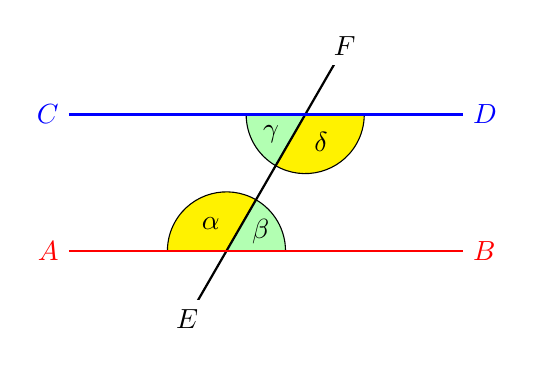
\begin{tikzpicture}
  \draw[fill=yellow] (0,0) -- (60:.75cm) arc (60:180:.75cm);
  \draw(120:0.4cm) node {$\alpha$};

  \draw[fill=green!30] (0,0) -- (right:.75cm) arc (0:60:.75cm);
  \draw(30:0.5cm) node {$\beta$};

  \begin{scope}[shift={(60:2cm)}]
    \draw[fill=green!30] (0,0) -- (180:.75cm) arc (180:240:.75cm);
    \draw (30:-0.5cm) node {$\gamma$};

    \draw[fill=yellow] (0,0) -- (240:.75cm) arc (240:360:.75cm);
    \draw (-60:0.4cm) node {$\delta$};
  \end{scope}

  \begin{scope}[thick]
    \draw (60:-1cm) node[fill=white] {$E$} -- (60:3cm) node[fill=white] {$F$};
    \draw[red]                   (-2,0) node[left] {$A$} -- (3,0) 
                                        node[right]{$B$};
    \draw[blue,shift={(60:2cm)}] (-3,0) node[left] {$C$} -- (2,0) 
                                        node[right]{$D$};
  \end{scope}
\end{tikzpicture}

Estimate the angles

\begin{tikzpicture}[scale=4,line width=1pt]                                    
  \coordinate (A) at (0,0);                                                    
  \coordinate (B) at ($(A)+(90:1)$);                                                    
  \coordinate (C) at ($(A)+(30:1)$);                                                
  \draw (A) -- (B);                                            
	\draw (A) -- (C);                                            
  \tikzMarkAngle{(A)}{(B)}{(C)}   
\end{tikzpicture}  

\begin{tikzpicture}[scale=4,line width=1pt]                                    
  \coordinate (A) at (0,0);                                                    
  \coordinate (B) at ($(A)+(90:1)$);                                                    
  \coordinate (C) at ($(A)+(0:1)$);                                                
  \draw (A) -- (B);                                            
	\draw (A) -- (C);                                            
  \tikzMarkAngle{(A)}{(B)}{(C)}   
\end{tikzpicture}  

\begin{tikzpicture}[scale=4,line width=1pt]                                    
  \coordinate (A) at (0,0);                                                    
  \coordinate (B) at ($(A)+(120:1)$);                                                    
  \coordinate (C) at ($(A)+(0:1)$);                                                
  \draw (A) -- (B);                                            
	\draw (A) -- (C);                                            
  \tikzMarkAngle{(A)}{(B)}{(C)}   
\end{tikzpicture}  

\begin{tikzpicture}[scale=4,line width=1pt]                                    
  \coordinate (A) at (0,0);                                                    
  \coordinate (B) at ($(A)+(-90:1)$);                                                    
  \coordinate (C) at ($(A)+(-135:1)$);                                                
  \draw (A) -- (B);                                            
	\draw (A) -- (C);                                            
  \tikzMarkAngle{(A)}{(B)}{(C)}   
\end{tikzpicture}  

\begin{tikzpicture}[scale=4,line width=1pt]                                    
  \coordinate (A) at (0,0);                                                    
  \coordinate (B) at ($(A)+(0:1)$);                                                    
  \coordinate (C) at ($(A)+(180:1)$);                                                
  \draw (A) -- (B);                                            
	\draw (A) -- (C);                                            
  \tikzMarkAngle{(A)}{(B)}{(C)}   
\end{tikzpicture}  

%parallelogram
\begin{tikzpicture}[scale=4,line width=1pt]                                    
  \coordinate (A) at (0,0);                                                    
  \coordinate (B) at (2,0);                                                    
  \coordinate (C) at ($(B)+(150:1)$);                                                
	\coordinate (D) at ($(A)+(150:1)$);                                                
  \draw (A) -- (B) -- (C) -- (D) -- cycle;                                            
	
  \tikzMarkAngle{(A)}{(B)}{(D)}   
	
	\tikzMarkAngle{(B)}{(A)}{(C)}
	
	\tikzMarkAngle{(C)}{(B)}{(D)}           
	\draw[shift={(D)}] (-30:0.15cm) arc (-30:0:0.15cm);      
\end{tikzpicture}  
\pagenumbering{gobble}
\tableofcontents
\newpage
%\listoftables
%\newpage
\listoffigures
\newpage
\listofalgorithms
\newpage
\setcounter{page}{0}
\pagenumbering{arabic}

\clearpage
\bibliographystyle{plain}
\bibliography{refs}

\begin{appendices}
	\chapter{Algorithms}
	%\begin{algorithm}
	\caption{Boilerplate}%\label{alg:euclid}
	\begin{algorithmic}[1]
		\Procedure{Boilerplate}{}
			\State \textbf{return} $4$\Comment{Random number decided by fair diceroll}
		\EndProcedure
	\end{algorithmic}
\end{algorithm}
	%\begin{algorithm}
	\caption{Euclids algorithms}\label{alg:euclid}
	\begin{algorithmic}[1]
		\Procedure{Euclid}{$a,b$}\Comment{The g.c.d of a and b}
			\State $r\gets a\bmod b$
			\While{$r\not=0$}\Comment{We have the answer if r is 0}
				\State $a\gets b$
				\State $b\gets r$
				\State $r\gets a\bmod b$
			\EndWhile\label{alg:euclid:endwhile}
			\State \textbf{return} $b$\Comment{The gcd is b}
		\EndProcedure
	\end{algorithmic}
\end{algorithm}
	\begin{algorithm}
	\caption{ID3}\label{alg:id3}
	\begin{algorithmic}[1]
		\Procedure{ID3}{$D$,$Attributes$,$Target$}
			\State $t\gets createNode()$
			\If{$\forall\langle x,c(x)\rangle \in D: c(x) = 1$}
				\State $t.label\gets 1$
				\State \textbf{return} $t$
			\ElsIf{$\forall\langle x,c(x)\rangle \in D: c(x) = 0$}
				\State $t.label\gets 0$
				\State \textbf{return} $t$
			\ElsIf{$Attributes = \emptyset$}
				\State $t.label\gets mostCommonClass(D, Target)$
				\State \textbf{return} $t$
			\Else
				\State $A^* = \argmax{A\in Attributes}IG(D, A)$
				\ForAll{$a\in A^*$}
					\State $D_a\gets\{(x,c(x))\in D : x\|_{A^*}=a\}$
					\If{$D_a = \emptyset$}
						\State $t'\gets createNode()$
						\State $t'.label = mostCommonClass(D, Target)$
						\State $createEdge(t, a, t')$
					\Else
						\State $createEdge(t, a, ID3(D_a, Attribute -\{A^*\}, Target))$
					\EndIf
				\EndFor
			\EndIf
			\State \textbf{return} $t$
		\EndProcedure
	\end{algorithmic}
\end{algorithm}
	\begin{algorithm}
	\caption{Basic K-means algorithm}\label{alg:kmeans}
	\begin{algorithmic}[1]
		%\Procedure{K-means}{K}
			\State Select $K$ points as inital centroids.
			\Repeat
				\State Form $K$ clusters by assigning each point to its closest centroid.
				\State Recompute the centroid of each cluster
			\Until Centroids do not change
		%\EndProcedure
	\end{algorithmic}
\end{algorithm}
	\begin{algorithm}
	\caption{Basic agglomerative hierarchical clustering algorihms.}\label{alg:agglomerative}
	\begin{algorithmic}[1]
			\State Compute the proximity matrix, if necessary.
			\Repeat
				\State Merge the closest two clusters.
				\State Update the proximity matrix to replect the proximity between the new cluster and the original clusters.
			\Until Only one cluster remains.
	\end{algorithmic}
\end{algorithm}
	\begin{algorithm}
	\caption{DBSCAN algorithms}\label{alg:dbscan}
	\begin{algorithmic}[1]
		\State Label all the point as core, border, or noise points.
		\State Eliminate noise points.
		\State Put an edge between all core points that are within $Eps$ of each other.
		\State Make each group of connected core points into a separate cluster.
		\State Assign each border point to one of the clusters of its associated core points.
	\end{algorithmic}
\end{algorithm}
		
\end{appendices}

\end{document}

